
\section{MCS Performance on Simulated Single Muons}\label{singlemuon_MC_section}

% Executive summary
In this section, MCS performance is studied on a sample of simulated, fully contained, single muons in {\ub}. It is demonstrated that the range-based energy of a track agrees with the true energy with negligible bias and with a resolution of better than 5\%. The MCS performance on single {\sc MCTracks} is shown to be comparable to that on single reconstructed PandoraNuPMA tracks when the track is well reconstructed, with a minimal bias and a resolution that varies between 5 and 20\%, performing better for higher energy (longer) tracks. Additionally, the scattering angle of track segments for a given energy is shown to be gaussian, in line with the Highland formula prediction both for {\sc MCTracks} and reconstructed tracks.


\subsection{Input Sample}\label{SingleMu_Input_Sample_section}
In order to study MCS performance in the most straightforward way, a sample of simulated single muons is used. This sample was generated in the {\ub} MCC7 production under the SAM definition ``prod\_muminus\_0-2.0GeV\_isotropic\_uboone\_mcc7\_reco2''. This sample consists of 19,500 single muons generated at a random location within the {\ub} TPC, with random direction. The energy spectrum of this sample is flat between 0 to 2 GeV kinetic energy of the muons. It is worth noting that the MCC7 simulation includes broken wires by masking specific channels on some planes in an attempt to better match real detector conditions (XXX reference about MCC7?).\\

This section of the technote will include studies from this single muon sample, both with {\sc MCTracks} (described in Section \ref{MCTrack_section}) and with reconstructed tracks (described in Section \ref{RecoTrack_section}).



%%%%%%%%%%%%%%%%%%%%%%%%%%%%%%%%%%%%%%%%%%%%%%%%%%%%%%%%%%%%%%%%%%%%%%%%%%%%%%%%%%%%%
\subsection{Performance with \sc{MCTracks}}


\subsubsection{MCTrack Description}\label{MCTrack_section}
{\sc MCTrack} objects are made from the output of {\sc geant}4, and are created from {\sc geant}4 energy depositions in the detector. {\sc geant}4 outputs 3D energy depositions in the detector, along with truth information about which parent particles deposited this energy. {\sc MCTracks} are 3D objects which are formed by grouping energy depositions based on parent particles. Whether a particle in {\sc geant}4 is turned into an {\sc MCTrack} or an {\sc MCShower} (not discussed in this note) is based on truth PDG (for example, muons always form {\sc MCTracks}).\\

Each {\sc MCTrack} is itself a vector of 3D trajectory points, which are ordered to match the direction of the particle that deposited the energy. Trajectory points are only formed for energy depositions inside of the TPC volume. In general, long {\sc MCTrack}s will have steps separated by up to several centimeters. Each step in an {\sc MCTrack} holds the following information used in this analysis: 3D position, and true energy at that point. Only information within the realm of reconstructable quantities is used in this analysis, with the exception of true energy (which is used for example to quantify a reconstructed energy resolution).\\

Since the output of a nominal reconstruction chain (going through hit finding, clustering, matching across planes, etc.) are 3D tracks, {\sc MCTracks} can be studied in an analysis in the exact same way as a reconstructed track would be. {\sc MCTracks} can be thought of as perfectly reconstructed tracks, where each trajectory point along the track is a true 3D energy deposition inside of the {\ub} TPC.\\

Since {\sc MCTracks} are formed from true 3D energy depositions and not from wire signals on drift electrons, {\sc MCTracks} are insensitive to broken wires, noise, and other simulated detector effects.

\subsubsection{MCTrack Selection}\label{MCTrack_Selection_section}
For analysis on single muon {\sc MCTracks}, the input sample is the one described in Section \ref{SingleMu_Input_Sample_section}. From that sample, the following requirements are placed for event selection:
\begin{enumerate}
	\item There is exactly one {\sc MCTrack} in the event
	\item The {\sc MCTrack} is longer than one meter in start-to-end length
	\item The {\sc MCTrack} is fully contained within the fiducial volume
	\item The {\sc MCTrack} does not decay in flight
\end{enumerate}
After these selection requirements are placed, the intial sample of 19,500 muons is reduced to 623 which are used for analysis.

\subsubsection{Range Energy Validation}\label{Range_Energy_Validation_section}
With this sample of {\sc MCTracks}, it is possible to quantify MCS energy resolution as a function of true energy. However, in actual {\ub} data there is obviously no true energy with which to compare. The additional energy handle that is used in data for contained tracks is range-based energy. The stopping power of muons in liquid argon is well described by the particle data group\cite{PDG_spline_table}. By using a linear interpolation between points in the cited PDG stopping power table, the start-to-end length of a track can be used to reconstruct the muon's total energy with good accuracy. Figure \ref{true_range_energy_MCTrack_fig} shows a comparison of range energy to true energy for this sample. \\

In order to compute a bias and a resolution, Figure \ref{true_range_energy_MCTrack_fig} is sliced in bins of true muon energy and a histogram of the fractional energy difference ($\frac{E_{range} - E_{true}}{E_{true}}$) is created for each bin. This distribution is shown for three representative bins in Figure \ref{true_range_bias_resolution_MCTrack_slices_fig}. The mean of each distribution is used to compute a bias a function of true energy, while the standard deviation of each distribution is used to compute a resolution. Figure \ref{true_range_bias_resolution_MCTrack_fig} shows the bias and resolution for this energy reconstruction method. It can be seen that the bias is negligible and the resolution for this method of energy reconstruction is on the order of 2-4\%. Based on this figure, it is clear that range-based energy is a good handle on the true energy of a reconstructed muon track in {\ub} data, assuming that track starts and ends near the true start and end of the muon.

\begin{figure}[h!]
\begin{center}
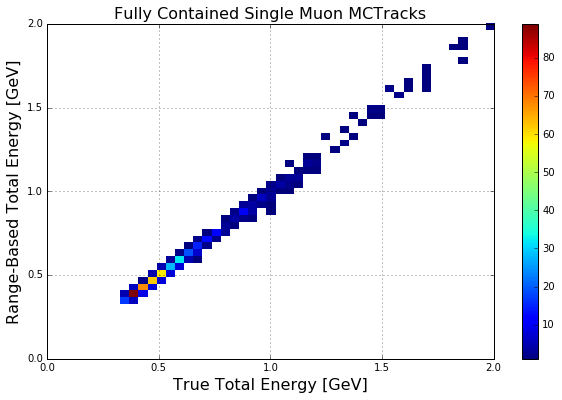
\includegraphics[width=100mm]{Figures/true_range_comparison_MCTracks.png}
\end{center}
\caption{\textit{Range based energy versus true energy for the single muon {\sc MCTrack} sample described in Section \ref{MCTrack_Selection_section}.}}
\label{true_range_energy_MCTrack_fig}
\end{figure}

\begin{figure}
\centering
\mbox{
	\subfigure[\textit{Fractional energy difference between 0.35 and 0.53 GeV true energy.}]
	{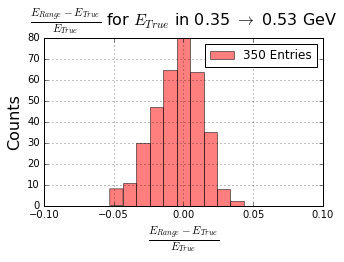
\includegraphics[width=50mm]{Figures/true_range_resolution_MCTracks_slice1.png}}
	\quad
	\subfigure[\textit{Fractional energy difference between 0.90 and 1.08 GeV true energy.}]
	{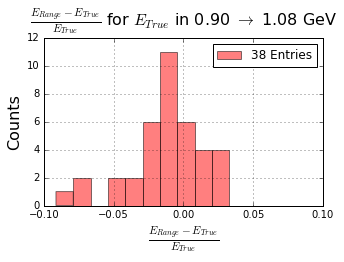
\includegraphics[width=50mm]{Figures/true_range_resolution_MCTracks_slice2.png}}
	\quad
	\subfigure[\textit{Fractional energy difference between 1.45 and 1.63 GeV true energy.}]
	{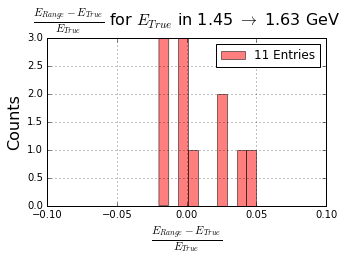
\includegraphics[width=50mm]{Figures/true_range_resolution_MCTracks_slice3.png}}
	}
\caption{\textit{Fractional energy difference for a few representative bins of true energy derived from Figure \ref{true_range_energy_MCTrack_fig}.}}
\label{true_range_bias_resolution_MCTrack_slices_fig}
\end{figure}




\begin{figure}
\centering
\mbox{
	\subfigure[\textit{Range energy bias as a function of true energy.}]
	{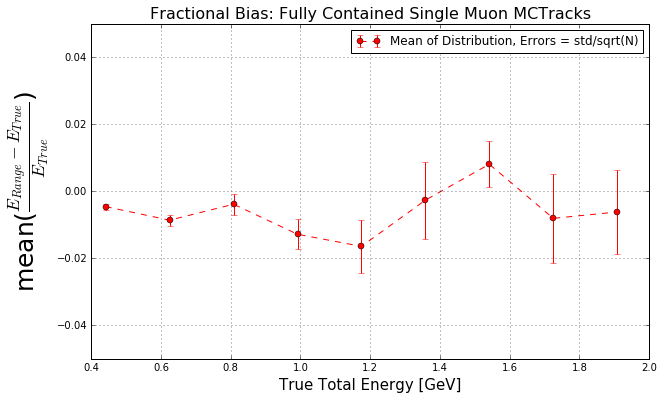
\includegraphics[width=75mm]{Figures/true_range_bias_MCTracks.png}}
	\quad
	\subfigure[\textit{Range energy resolution as a function of true energy.}]
	{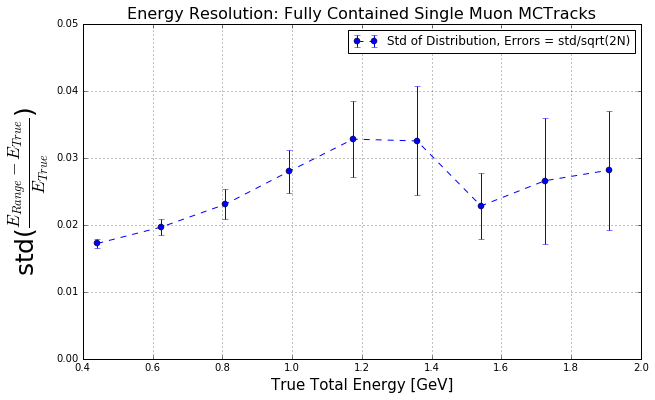
\includegraphics[width=75mm]{Figures/true_range_resolution_MCTracks.png}}
	}
\caption{\textit{Range energy and true energy bias and resolution for the single muon {\sc MCTrack} sample described in Section \ref{MCTrack_Selection_section}.}}
\label{true_range_bias_resolution_MCTrack_fig}
\end{figure}




\subsubsection{MCS Energy Validation}\label{MCS_Energy_Validation_MCTrack_section}
For this sample of {\sc MCTracks}, the trajectory points only of each {\sc MCTrack} is used as input to the MCS code, described in Section XXX. The resulting MCS energy versus range-based energy can be seen in Figure \ref{MCS_range_energy_MCTrack_fig}. Range energy is used here instead of true energy in order to make this plot more directly comparable with the same analysis on data where true energy is not accessible\footnote{It is acceptable to use range energy based on Figure \ref{true_range_bias_resolution_MCTrack_fig}.}. In order to compute a bias and a resolution, Figure \ref{MCS_range_energy_MCTrack_fig} is sliced in bins of range energy and a histogram of the fractional energy difference ($\frac{E_{MCS} - E_{range}}{E_{range}}$) is created for each bin. This distribution is shown for three representative bins in Figure \ref{MCS_range_bias_resolution_MCTrack_slices_fig}. The mean of each distribution is used to compute a bias a function of range energy, while the standard deviation of each distribution is used to compute a resolution. The bias and resolution for this energy reconstruction method shown in Figure \ref{MCS_range_bias_resolution_MCTrack_fig}. This figure indicates a bias in the MCS energy resolution on the order of a few percent, with a resolution that decreases from about 18\% for contained {\sc MCTracks} with true total energy around 0.5 GeV (which corresponds to a length of about 1.7 meters) to below 10\% for contained {\sc MCTracks} with true total energy greater than 0.8 GeV (which corresponds to a length of about 3.1 meters).


\begin{figure}[h!]
\begin{center}
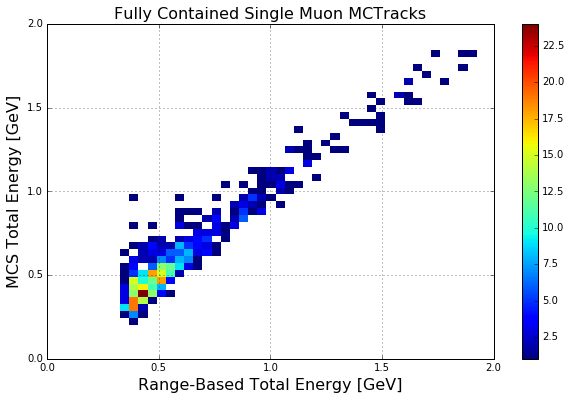
\includegraphics[width=100mm]{Figures/MCS_range_comparison_MCTracks.png}
\end{center}
\caption{\textit{MCS computed energy versus range energy for the single muon {\sc MCTrack} sample described in Section \ref{MCTrack_Selection_section}.}}
\label{MCS_range_energy_MCTrack_fig}
\end{figure}

\begin{figure}
\centering
\mbox{
	\subfigure[\textit{Fractional energy difference between 0.35 and 0.53 GeV range energy.}]
	{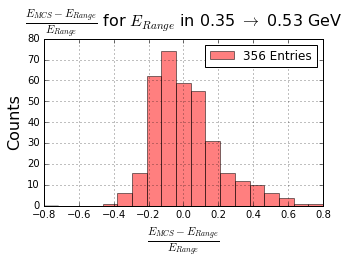
\includegraphics[width=50mm]{Figures/MCS_range_resolution_MCTracks_slice1.png}}
	\quad
	\subfigure[\textit{Fractional energy difference between 0.90 and 1.08 GeV range energy.}]
	{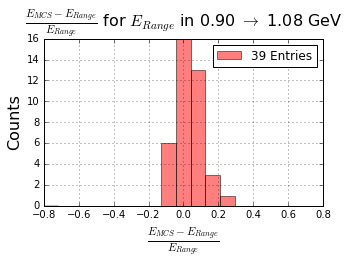
\includegraphics[width=50mm]{Figures/MCS_range_resolution_MCTracks_slice2.png}}
	\quad
	\subfigure[\textit{Fractional energy difference between 1.45 and 1.63 GeV range energy.}]
	{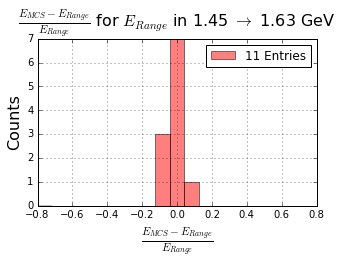
\includegraphics[width=50mm]{Figures/MCS_range_resolution_MCTracks_slice3.png}}
	}
\caption{\textit{Fractional energy difference for a few representative bins of range energy derived from Figure \ref{MCS_range_energy_MCTrack_fig}.}}
\label{MCS_range_bias_resolution_MCTrack_slices_fig}
\end{figure}


\begin{figure}
\centering
\mbox{
	\subfigure[\textit{MCS energy bias as a function of range energy.}]
	{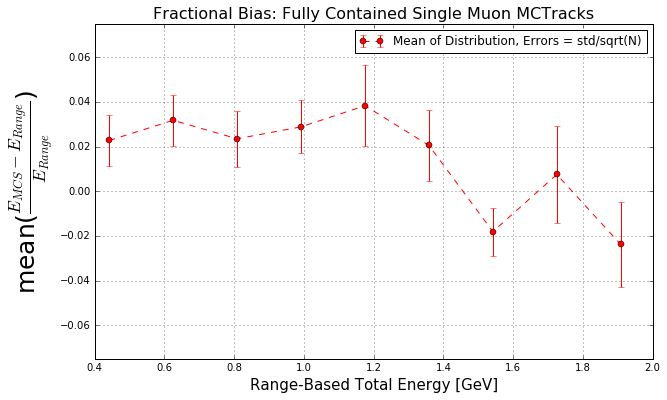
\includegraphics[width=75mm]{Figures/MCS_range_bias_MCTracks.png}}
	\quad
	\subfigure[\textit{MCS energy resolution as a function of range energy.}]
	{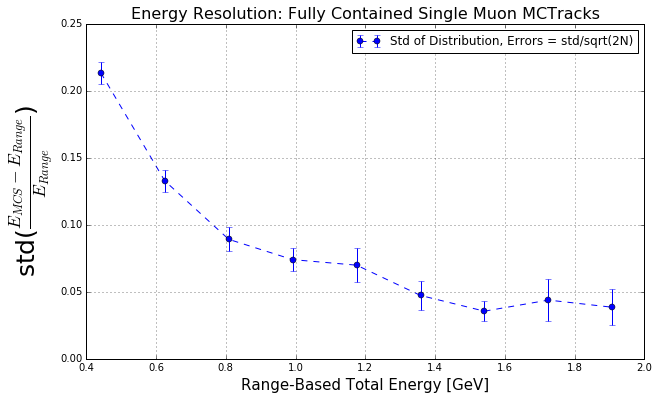
\includegraphics[width=75mm]{Figures/MCS_range_resolution_MCTracks.png}}
	}
\caption{\textit{MCS energy bias and resolution as a function of range energy for the single muon {\sc MCTrack} sample described in Section \ref{MCTrack_Selection_section}.}}
\label{MCS_range_bias_resolution_MCTrack_fig}
\end{figure}



\subsubsection{Highland Validation}\label{Highland_Validation_MCTrack_section}
For a given track segment energy and length, 98\% of the angular scatter deviations should be gaussian with an RMS described by the Highland equation (Equation \ref{highland_eqtn}), while the remaining 2\% are larger angle Rutherford scatters [XXX source]. Therefore, a histogram of track segment angular deviations divided by the RMS predicted by the Highland equation should be gaussian with a width of unity. In this section, we validate this claim.\\

For each 20cm segment of each {\sc MCTrack} in this single muon sample, the energy of the muon at the start of that segment is estimated by taking the computed MCS energy and subtracting out energy lost in the track upstream of the start of this segment, assuming the track was minimally ionizing (depositing 2.2 MeV per centimeter of track). This energy, along with the segment length, is converted into an expected RMS angular deviation by way of Equation \ref{highland_eqtn}. For each consecutive pairs of segments, the angular scatter in milliradians divided by the Highland expected RMS in millradians is an entry in the histogram shown in Figure \ref{Highland_validation_MCTracks_fig}. From this figure we can see that the Highland formula is valid for {\sc MCTracks}.

\begin{figure}[h!]
\begin{center}
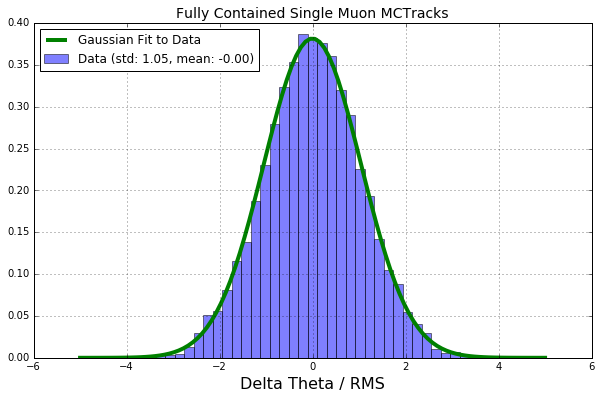
\includegraphics[width=100mm]{Figures/Highland_validation_MCTracks.png}
\end{center}
\caption{\textit{20cm segment angular deviations divided by expected Highland RMS for the single muon {\sc MCTrack} sample described in Section \ref{MCTrack_Selection_section}.}}
\label{Highland_validation_MCTracks_fig}
\end{figure}













%%%%%%%%%%%%%%%%%%%%%%%%%%%%%%%%%%%%%%%%%%%%%%%%%%%%%%%%%%%%%%%%%%%%%%%%%%%%%%%%%%%%%

\subsection{Performance with Reconstructed Tracks}
\subsubsection{Reconstructed Track Description}\label{RecoTrack_section}
XXX this section has description of PandoraNuPMA tracks, cite pandora reference rather than lengthy description.

\subsubsection{Reconstructed Track Selection}\label{RecoTrack_Selection_section}
For analysis on single muon reconstructed tracks, the input sample is the one described in Section \ref{SingleMu_Input_Sample_section}. From that sample, the requirements described in Section \ref{MCTrack_Selection_section} are first placed on the sample. Then, the following additional requirements are placed for event selection:
\begin{enumerate}
	\item There is exactly one reconstructed track in the event
	\item The reconstructed track is longer than one meter in start-to-end length
	\item The reconstructed track is fully contained within the fiducial volume
	\item The start of the reconstructed track is within 3cm of the start of the {\sc MCTrack}, and the end of the reconstructed track is within 3cm of the end of the {\sc MCTrack} (or vice-versa).
\end{enumerate}
The last selection criteria is the one most worth noting; it ensures that the track is well reconstructed and not broken or truncated. The purpose the ``vice-versa'' claus in the last selection criteria is to take into account tracks that are well reconstructed in terms of position, but are flipped in direction. In the case of backwards-tracks, the reconstructed track is flipped to have the correct direction before proceeding with the analysis. The application of these track selection cuts reduces the sample down to 307 reconstructed single muon tracks, which are used in this analysis.






\subsubsection{MCS Energy Validation}\label{MCS_Energy_Validation_MCTrack_section}
For this sample of reconstructed tracks, the trajectory points only of each track is used as input to the MCS code, described in Section XXX. The resulting MCS energy versus range-based energy can be seen in Figure \ref{MCS_range_energy_RecoTrack_fig}. In order to compute a bias and a resolution, Figure \ref{MCS_range_energy_RecoTrack_fig} is sliced in bins of range energy and a histogram of the fractional energy difference ($\frac{E_{MCS} - E_{range}}{E_{range}}$) is created for each bin. This distribution is shown for three representative bins in Figure \ref{MCS_range_bias_resolution_RecoTrack_slices_fig}. The mean of each distribution is used to compute a bias a function of range, while the standard deviation of each distribution is used to compute a resolution. The bias and resolution for this energy reconstruction method shown in Figure \ref{MCS_range_bias_resolution_RecoTrack_fig}. XXX CHECK THIS XXX This figure indicates a bias in the MCS energy resolution on the order of a few percent, with a resolution that decreases from about 18\% for contained {\sc MCTracks} with true total energy around 0.5 GeV (which corresponds to a length of about 1.7 meters) to below 10\% for contained {\sc MCTracks} with true total energy greater than 0.8 GeV (which corresponds to a length of about 3.1 meters).


\begin{figure}[h!]
\begin{center}
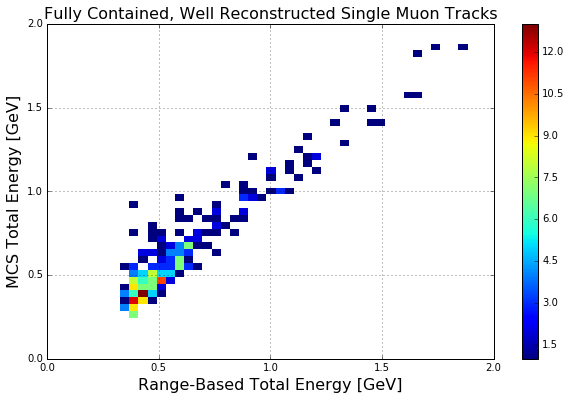
\includegraphics[width=100mm]{Figures/MCS_range_comparison_RecoTracks.png}
\end{center}
\caption{\textit{MCS computed energy versus range energy for the single muon reconstructed track sample described in Section \ref{RecoTrack_Selection_section}.}}
\label{MCS_range_energy_RecoTrack_fig}
\end{figure}

\begin{figure}
\centering
\mbox{
	\subfigure[\textit{Fractional energy difference between 0.35 and 0.53 GeV range energy.}]
	{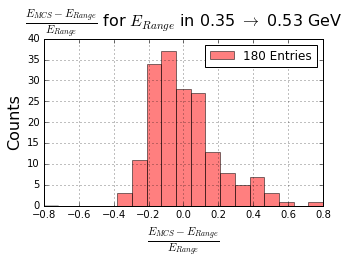
\includegraphics[width=50mm]{Figures/MCS_range_resolution_RecoTracks_slice1.png}}
	\quad
	\subfigure[\textit{Fractional energy difference between 0.90 and 1.08 GeV range energy.}]
	{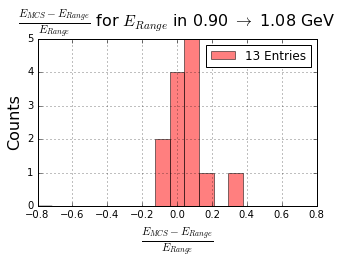
\includegraphics[width=50mm]{Figures/MCS_range_resolution_RecoTracks_slice2.png}}
	\quad
	\subfigure[\textit{Fractional energy difference between 1.45 and 1.63 GeV range energy.}]
	{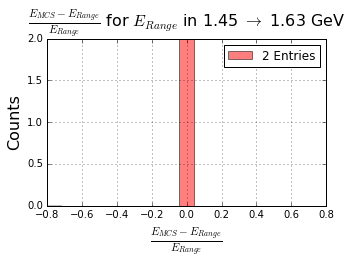
\includegraphics[width=50mm]{Figures/MCS_range_resolution_RecoTracks_slice3.png}}
	}
\caption{\textit{Fractional energy difference for a few representative bins of range energy derived from Figure \ref{MCS_range_energy_RecoTrack_fig}.}}
\label{MCS_range_bias_resolution_RecoTrack_slices_fig}
\end{figure}


\begin{figure}
\centering
\mbox{
	\subfigure[\textit{MCS energy bias as a function of range energy.}]
	{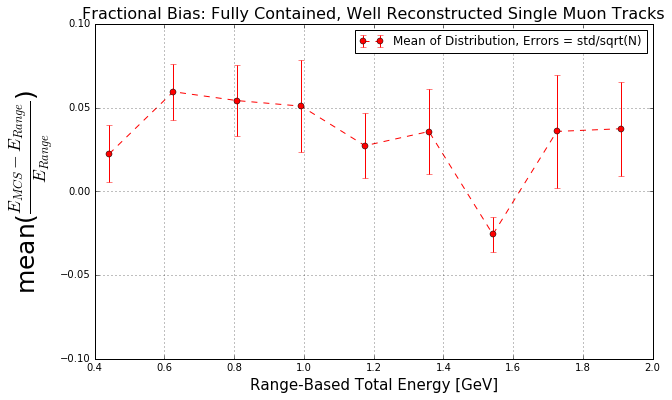
\includegraphics[width=75mm]{Figures/MCS_range_bias_RecoTracks.png}}
	\quad
	\subfigure[\textit{MCS energy resolution as a function of range energy.}]
	{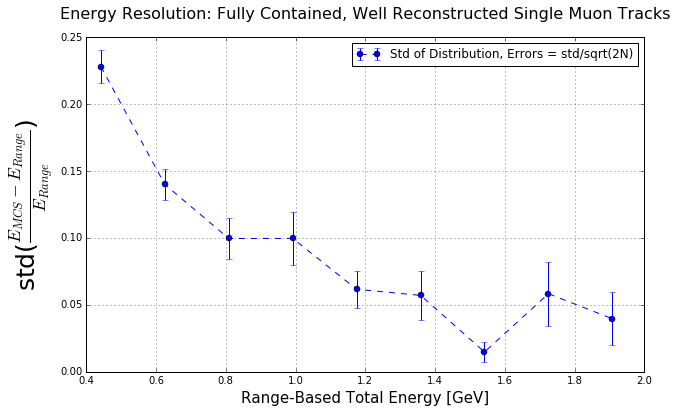
\includegraphics[width=75mm]{Figures/MCS_range_resolution_RecoTracks.png}}
	}
\caption{\textit{MCS energy bias and resolution as a function of range energy for the single muon reconstructed track sample described in Section \ref{RecoTrack_Selection_section}.}}
\label{MCS_range_bias_resolution_RecoTrack_fig}
\end{figure}



\subsubsection{Highland Validation}\label{Highland_Validation_RecoTrack_section}
For a given track segment energy and length, 98\% of the angular scatter deviations should be gaussian with an RMS described by the Highland equation (Equation \ref{highland_eqtn}), while the remaining 2\% are larger angle Rutherford scatters [XXX source]. Therefore, a histogram of track segment angular deviations divided by the RMS predicted by the Highland equation should be gaussian with a width of unity. In this section, we validate this claim.\\

For each 20cm segment of each reconstructed track in this single muon sample, the energy of the muon at the start of that segment is estimated by taking the computed MCS energy and subtracting out energy lost in the track upstream of the start of this segment, assuming the track was minimally ionizing (depositing 2.2 MeV per centimeter of track). This energy, along with the segment length, is converted into an expected RMS angular deviation by way of Equation \ref{highland_eqtn}. For each consecutive pairs of segments, the angular scatter in milliradians divided by the Highland expected RMS in millradians is an entry in the histogram shown in Figure \ref{Highland_validation_RecoTracks_fig}. From this figure we can see that the Highland formula is valid for reconstructed tracks, though the width is slightly smaller than unity. XXX maybe make a statement here about ``track straightening''?

\begin{figure}[h!]
\begin{center}
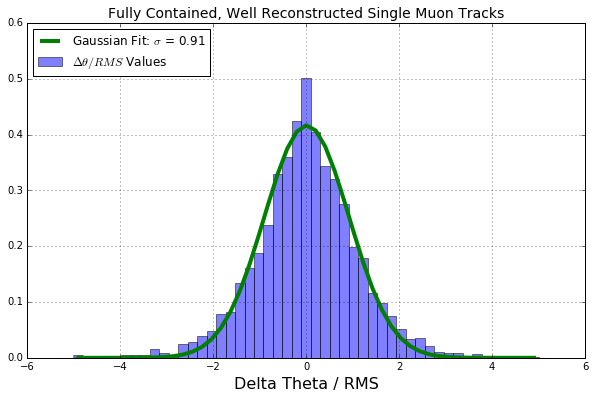
\includegraphics[width=100mm]{Figures/Highland_validation_RecoTracks.png}
\end{center}
\caption{\textit{20cm segment angular deviations divided by expected Highland RMS for the single muon reconstructed track sample described in Section \ref{RecoTrack_Selection_section}.}}
\label{Highland_validation_RecoTracks_fig}
\end{figure}


















% \subsection{Track Reconstruction and Event Selection}
% \subsubsection{Reconstructed Track Description}\label{RecoTrack_section}
% \begin{enumerate}
% \item brief description of pandoraNuPMA algorithm, reference to pandora neutrino2016 documentation
% \item We select events with 1 reconstructed track longer than 1 meter that starts and ends in the correct place (including reversed direction, which we take into account)... correct place means within 5cm of true start and end.
% \item plot of scattering angle / RMS (RMS from range energy)
% \item plot of MCS energy vs true energy
% \item energy resolution in terms of true energy
% \item energy resolution in terms of range energy
% \end{enumerate}

% \subsection{Optimizing Segment Length}
% \begin{enumerate}
% \item using the reconstructed tracks in previous section, overlay energy resolution vs true energy for different segment lengths to pick the best one
% \item also show angle/RMS plot for different segment lengths to show that it only becomes gaussian for longer segment lengths, and that is motivation to pick longer segment lengths.
% \end{enumerate}

% \subsection{Exiting Tracks}
% \begin{enumerate}
% \item reminder that the primary purpose of MCS is to get the energy of exiting tracks
% \item in this section we will use MCTracks that start in fiducial volume and end somewhere outside of it
% \item plot of MCS energy vs true energy
% \item plot: energy resolution in terms of true energy
% \item plot: energy resolution in terms of length of track contained
% \item plot: 2D energy resolution in terms of true energy and length of track contained? dunno if enough stats for that
% \end{enumerate}

% \subsection{MCS as a Tool to Determine Track Direction}
% \begin{enumerate}
% \item here we talk about running MCS on single muon contined reco tracks backwards and forwards and show the likelihood is better for forwards.
% \item i think bruce worked on this first... cite his DocDB about it?
% \end{enumerate}

% \subsection{MCS as a Tool to Determine Reconstruction Quality}
% \begin{enumerate}
% \item here we talk about how broken tracks are a problem, and we show the MCS vs range energy for reco tracks that are broken, and for ones that are not broken, and show that if MCS energy doesn't match range energy one can say that the track is poorly reconstructed.
% \end{enumerate}

% \subsection{MCS as a Tool for Pion/Muon Separation}
% \begin{enumerate}
% \item this is a potential section where we run on pions and muons and somehow claim that MCS can work to separate the two to some extent
% \end{enumerate}


